\section{Date: 2024-10-11}
\noindent \textbf{Series ID: BNEMFT01KRQ460S} 

\noindent This series is titled Business Tendency Surveys for Non-Manufacturing: Employment: Future Tendency: National Indicator for the Republic of Korea (DISCONTINUED) and has a frequency of Quarterly. The units are Net Percent and the seasonal adjustment is Seasonally Adjusted.The observation start date is 1993-01-01 and the observation end date is 2003-01-01.The popularity of this series is 1. \\ 

\noindent \textbf{Series ID: THREEFFTP6} 

\noindent This series is titled Instantaneous Forward Term Premium 6 Years Hence and has a frequency of Daily. The units are Percent and the seasonal adjustment is Not Seasonally Adjusted.The observation start date is 1990-01-02 and the observation end date is 2024-10-04.The popularity of this series is 2. \\ 

\subsection{Regression Tables and Plots}
\begin{center}
\begin{tabular}{lclc}
\toprule
\textbf{Dep. Variable:}               & value\_fred\_THREEFFTP6 & \textbf{  R-squared:         } &     0.488   \\
\textbf{Model:}                       &           OLS           & \textbf{  Adj. R-squared:    } &     0.459   \\
\textbf{Method:}                      &      Least Squares      & \textbf{  F-statistic:       } &     17.14   \\
\textbf{Date:}                        &     Fri, 11 Oct 2024    & \textbf{  Prob (F-statistic):} &  0.000614   \\
\textbf{Time:}                        &         14:58:58        & \textbf{  Log-Likelihood:    } &   -3.4076   \\
\textbf{No. Observations:}            &              20         & \textbf{  AIC:               } &     10.82   \\
\textbf{Df Residuals:}                &              18         & \textbf{  BIC:               } &     12.81   \\
\textbf{Df Model:}                    &               1         & \textbf{                     } &             \\
\textbf{Covariance Type:}             &        nonrobust        & \textbf{                     } &             \\
\bottomrule
\end{tabular}
\begin{tabular}{lcccccc}
                                      & \textbf{coef} & \textbf{std err} & \textbf{t} & \textbf{P$> |$t$|$} & \textbf{[0.025} & \textbf{0.975]}  \\
\midrule
\textbf{const}                        &       1.3795  &        0.088     &    15.636  &         0.000        &        1.194    &        1.565     \\
\textbf{value\_fred\_BNEMFT01KRQ460S} &      -0.0328  &        0.008     &    -4.140  &         0.001        &       -0.049    &       -0.016     \\
\bottomrule
\end{tabular}
\begin{tabular}{lclc}
\textbf{Omnibus:}       &  2.364 & \textbf{  Durbin-Watson:     } &    1.557  \\
\textbf{Prob(Omnibus):} &  0.307 & \textbf{  Jarque-Bera (JB):  } &    0.806  \\
\textbf{Skew:}          & -0.193 & \textbf{  Prob(JB):          } &    0.668  \\
\textbf{Kurtosis:}      &  3.905 & \textbf{  Cond. No.          } &     14.6  \\
\bottomrule
\end{tabular}
%\caption{OLS Regression Results}
\end{center}

Notes: \newline
 [1] Standard Errors assume that the covariance matrix of the errors is correctly specified.

\begin{figure}
\centering
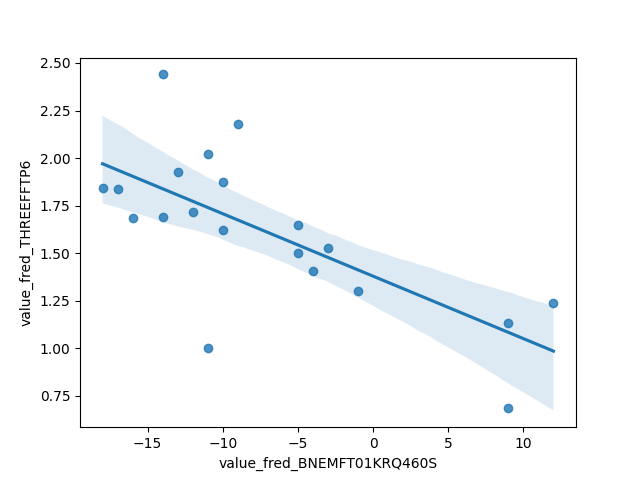
\includegraphics[scale = 0.9]{plots/plot_2024-10-11.png}
\caption{Regression Plot for 2024-10-11}
\end{figure}
\newpage
